\documentclass[12pt, twoside]{article}
\usepackage[francais]{babel}
\usepackage[T1]{fontenc}
\usepackage[latin1]{inputenc}
\usepackage[left=7mm, right=1cm, top=1cm, bottom=7mm]{geometry}
\usepackage{float}
\usepackage{graphicx}
\usepackage{array}
\usepackage{multirow}
\usepackage{amsmath,amssymb,mathrsfs}
\usepackage{soul}
\usepackage{textcomp}
\usepackage{eurosym}
\usepackage{variations}
\usepackage{tabvar}

\begin{document}


\ul{Exercice} : 
Nommer les triangles rectangles � l'aide des points marqu�s sur les figures suivantes. (Tous les c�t�s des triangles �
rep�rer ne sont pas forc�ment trac�s.) Dans chaque cas le centre du cercle est le point $O$.
\begin{center}
	\begin{tabular}{cccc}
			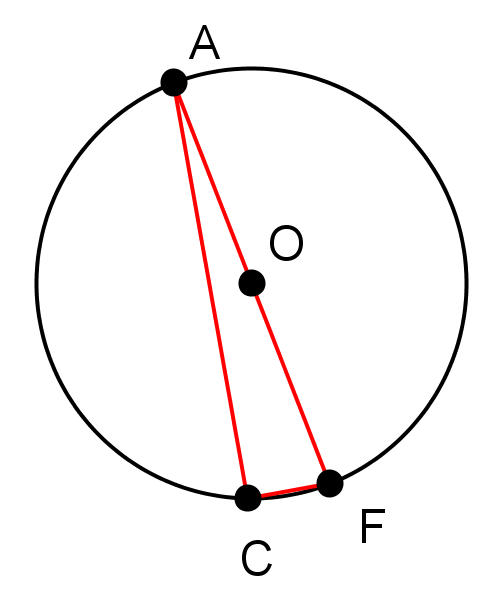
\includegraphics[width=3.2cm]{images/cercle01.png}
	&
			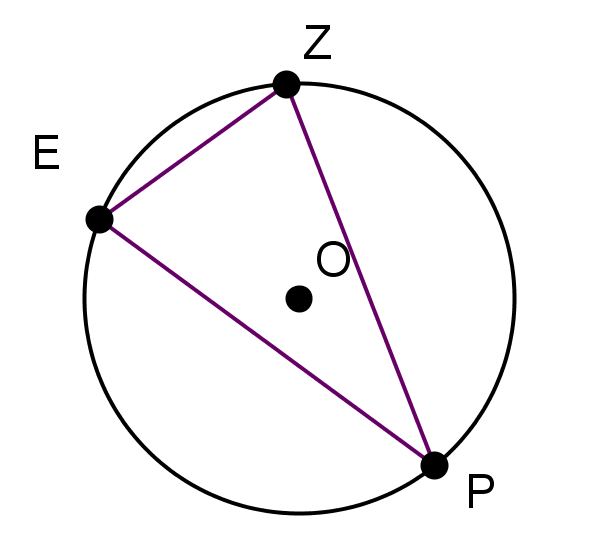
\includegraphics[width=4cm]{images/cercle02.png}
	&
			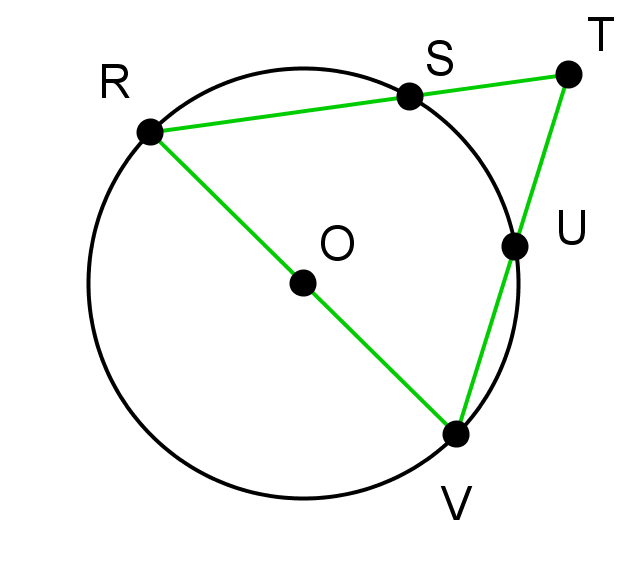
\includegraphics[width=4cm]{images/cercle03.png}
	&
			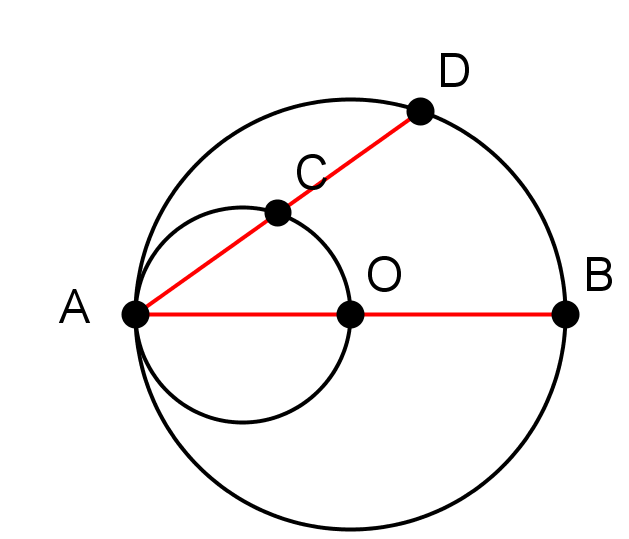
\includegraphics[width=4cm]{images/cercle04.png}
	\end{tabular}
\end{center}
\ul{Exercice} : 
Nommer les triangles rectangles � l'aide des points marqu�s sur les figures suivantes. (Tous les c�t�s des triangles �
rep�rer ne sont pas forc�ment trac�s.) Dans chaque cas le centre du cercle est le point $O$.
\begin{center}
	\begin{tabular}{cccc}
			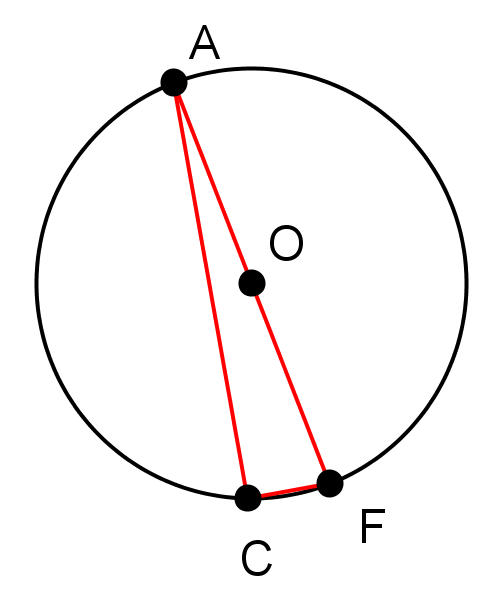
\includegraphics[width=3.2cm]{images/cercle01.png}
	&
			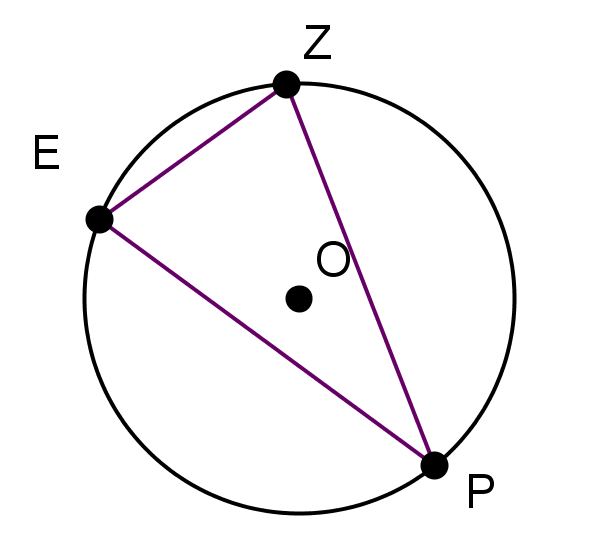
\includegraphics[width=4cm]{images/cercle02.png}
	&
			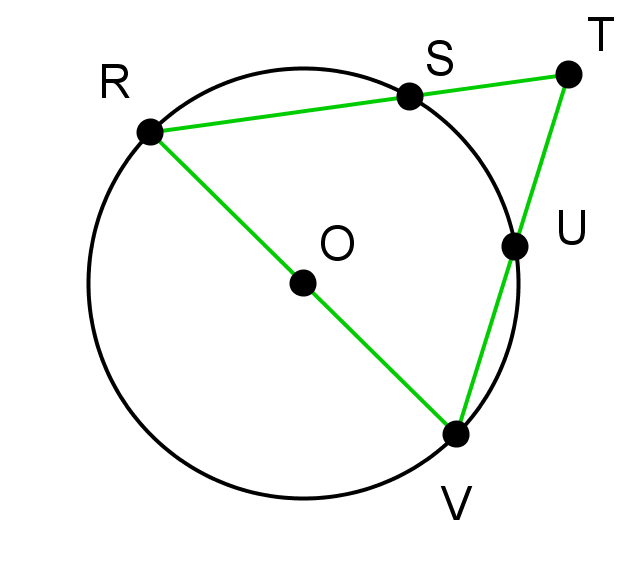
\includegraphics[width=4cm]{images/cercle03.png}
	&
			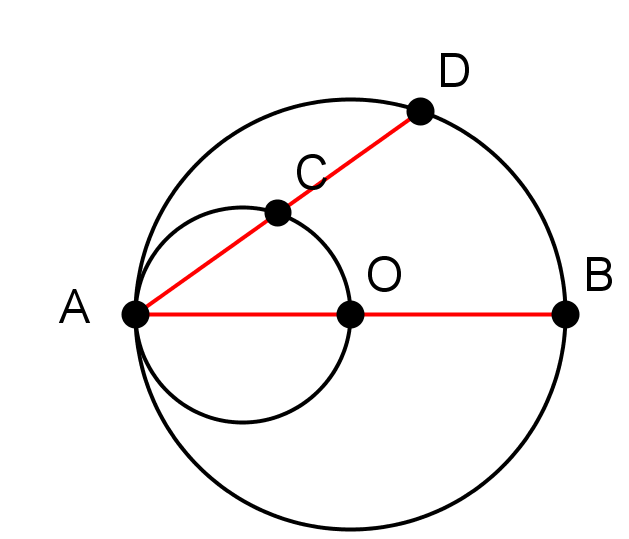
\includegraphics[width=4cm]{images/cercle04.png}
	\end{tabular}
\end{center}

\bigskip

\ul{Exercice} : 
Nommer les triangles rectangles � l'aide des points marqu�s sur les figures suivantes. (Tous les c�t�s des triangles �
rep�rer ne sont pas forc�ment trac�s.) Dans chaque cas le centre du cercle est le point $O$.
\begin{center}
	\begin{tabular}{cccc}
			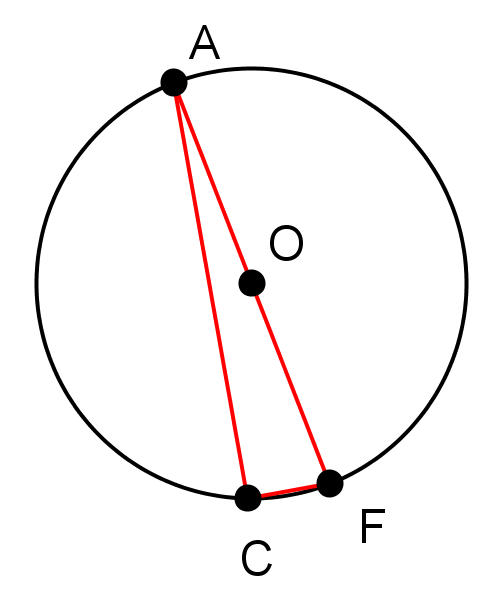
\includegraphics[width=3.2cm]{images/cercle01.png}
	&
			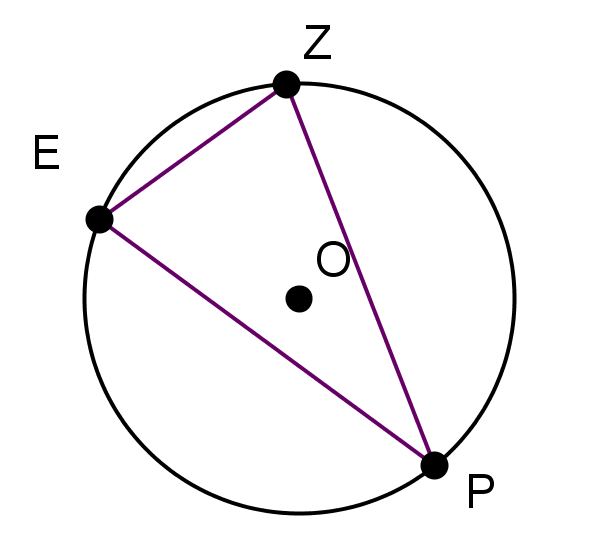
\includegraphics[width=4cm]{images/cercle02.png}
	&
			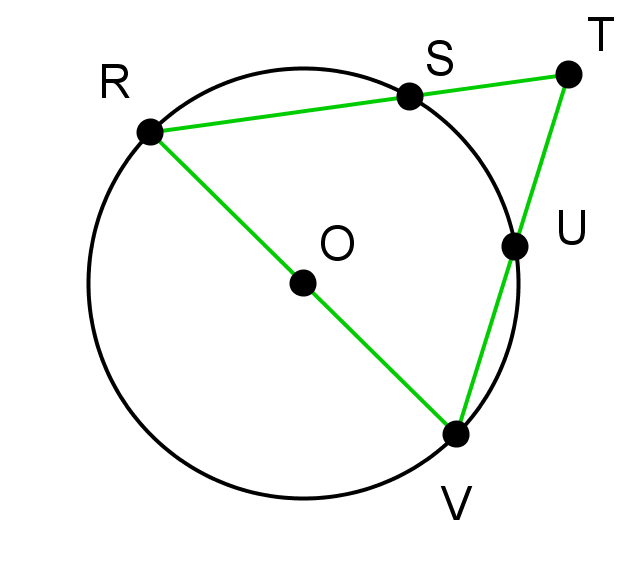
\includegraphics[width=4cm]{images/cercle03.png}
	&
			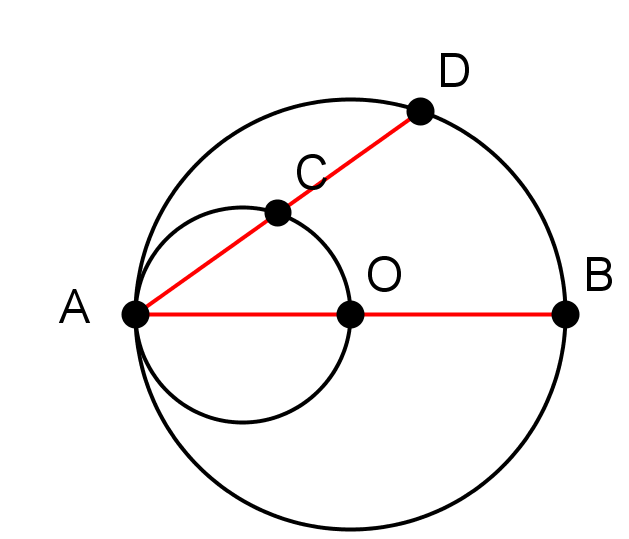
\includegraphics[width=4cm]{images/cercle04.png}
	\end{tabular}
\end{center}


\bigskip
\ul{Exercice} : 
Nommer les triangles rectangles � l'aide des points marqu�s sur les figures suivantes. (Tous les c�t�s des triangles �
rep�rer ne sont pas forc�ment trac�s.) Dans chaque cas le centre du cercle est le point $O$.
\begin{center}
	\begin{tabular}{cccc}
			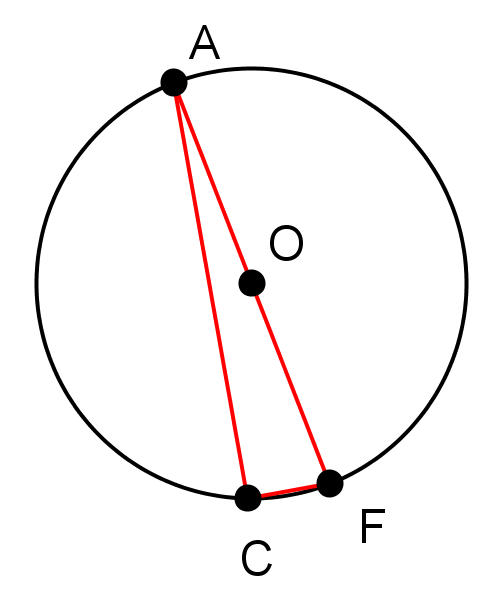
\includegraphics[width=3.2cm]{images/cercle01.png}
	&
			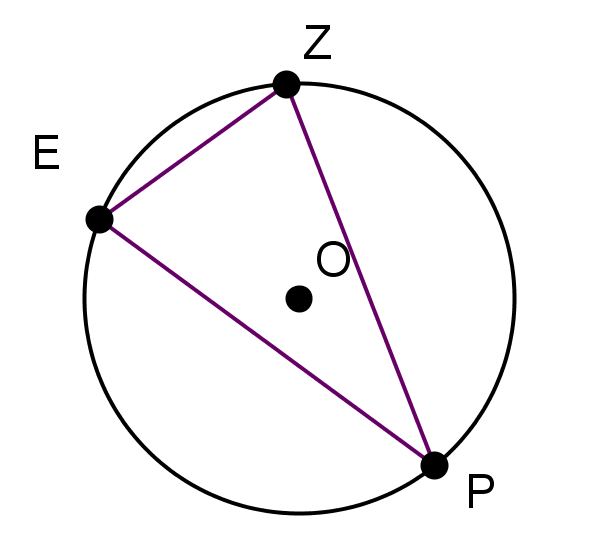
\includegraphics[width=4cm]{images/cercle02.png}
	&
			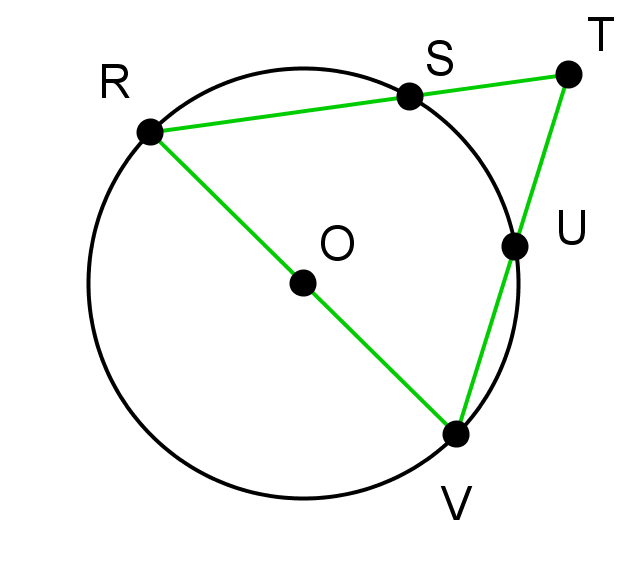
\includegraphics[width=4cm]{images/cercle03.png}
	&
			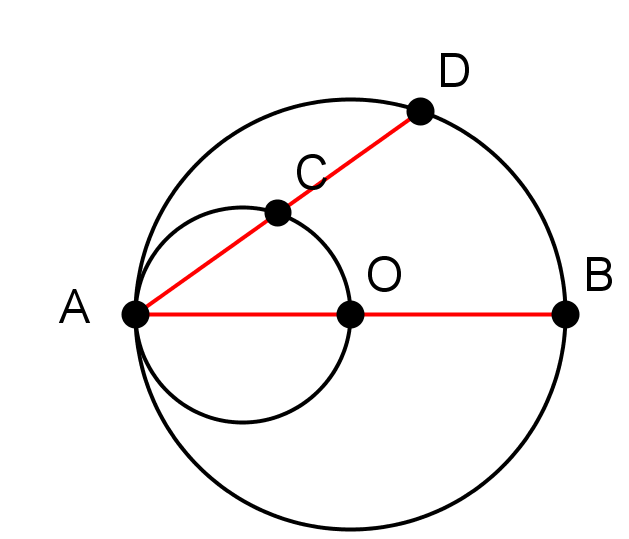
\includegraphics[width=4cm]{images/cercle04.png}
	\end{tabular}
\end{center}


\end{document}
